%%
%% This is file `sample-sigconf.tex',
%% generated with the docstrip utility.
%%
%% The original source files were:
%%
%% samples.dtx  (with options: `sigconf')
%%
%% IMPORTANT NOTICE:
%%
%% For the copyright see the source file.
%%
%% Any modified versions of this file must be renamed
%% with new filenames distinct from sample-sigconf.tex.
%%
%% For distribution of the original source see the terms
%% for copying and modification in the file samples.dtx.
%%
%% This generated file may be distributed as long as the
%% original source files, as listed above, are part of the
%% same distribution. (The sources need not necessarily be
%% in the same archive or directory.)
%%
%% The first command in your LaTeX source must be the \documentclass command.
\documentclass[sigplan,10pt,anonymous,review]{acmart}

\providecommand{\tightlist}{%
  \setlength{\itemsep}{0pt}\setlength{\parskip}{0pt}}

%%
%% \BibTeX command to typeset BibTeX logo in the docs
\AtBeginDocument{%
  \providecommand\BibTeX{{%
    \normalfont B\kern-0.5em{\scshape i\kern-0.25em b}\kern-0.8em\TeX}}}

%% Rights management information.  This information is sent to you
%% when you complete the rights form.  These commands have SAMPLE
%% values in them; it is your responsibility as an author to replace
%% the commands and values with those provided to you when you
%% complete the rights form.

%%
%% Submission ID.
%% Use this when submitting an article to a sponsored event. You'll
%% receive a unique submission ID from the organizers
%% of the event, and this ID should be used as the parameter to this command.
%%\acmSubmissionID{123-A56-BU3}

%%
%% The majority of ACM publications use numbered citations and
%% references.  The command \citestyle{authoryear} switches to the
%% "author year" style.
%%
%% If you are preparing content for an event
%% sponsored by ACM SIGGRAPH, you must use the "author year" style of
%% citations and references.
%% Uncommenting
%% the next command will enable that style.
%%\citestyle{acmauthoryear}

%%
%% end of the preamble, start of the body of the document source.
\begin{document}

%%
%% The "title" command has an optional parameter,
%% allowing the author to define a "short title" to be used in page headers.
\title{Customizing Software by Direct Manipulation of Tabular Data}

%%
%% The "author" command and its associated commands are used to define
%% the authors and their affiliations.
%% Of note is the shared affiliation of the first two authors, and the
%% "authornote" and "authornotemark" commands
%% used to denote shared contribution to the research.

\author{Geoffrey Litt}
\affiliation{%
  \institution{Massachusetts Institute of Technology}
  \city{Cambridge, MA}
  \country{USA}
}
\email{glitt@mit.edu}

\author{Daniel Jackson}
\affiliation{%
  \institution{Massachusetts Institute of Technology}
  \city{Cambridge, MA}
  \country{USA}
}
\email{dnj@csail.mit.edu}

%%
%% By default, the full list of authors will be used in the page
%% headers. Often, this list is too long, and will overlap
%% other information printed in the page headers. This command allows
%% the author to define a more concise list
%% of authors' names for this purpose.
% \renewcommand{\shortauthors}{Trovato and Tobin, et al.}

%%
%% The abstract is a short summary of the work to be presented in the
%% article.
\begin{abstract}
  In this paper we show how the behavior of a software application can
  be extended and adapted by direct manipulation, using table-driven
  customization, a new paradigm that allows end users to customize
  applications without writing traditional code.

  Instead, users directly manipulate a tabular view of the structured
  data inside the application---rather than writing imperative scripts
  (as in most customization tools). This simple model also accommodates
  a spreadsheet formula language and custom data editing widgets, which
  provide sufficient expressivity to implement many useful
  customizations.

  We illustrate the approach with Wildcard, a browser extension that
  implements table-driven customization in the context of web
  applications. Through concrete examples, we show that our paradigm can
  be used to create useful customizations for real applications. We
  share reflections from experience using the Wildcard system, on both
  its strengths and limitations relative to other customization
  approaches. Finally, we explore how this paradigm might lead to new
  software architectures that encourage this form of customization.
\end{abstract}

%%
%% The code below is generated by the tool at http://dl.acm.org/ccs.cfm.
%% Please copy and paste the code instead of the example below.
%%
%% From HERE
\begin{CCSXML}
<ccs2012>
<concept>
<concept_id>10011007.10011006.10011066.10011069</concept_id>
<concept_desc>Software and its engineering~Integrated and visual development environments</concept_desc>
<concept_significance>500</concept_significance>
</concept>
</ccs2012>
\end{CCSXML}

\ccsdesc[500]{Software and its engineering~Integrated and visual development environments}
% To HERE

%%
%% Keywords. The author(s) should pick words that accurately describe
%% the work being presented. Separate the keywords with commas.
\keywords{end-user programming, software customization, web browser extensions}

%% A "teaser" image appears between the author and affiliation
%% information and the body of the document, and typically spans the
%% page.
%\begin{teaserfigure}
%  \includegraphics[width=\textwidth]{sampleteaser}
%  \caption{Seattle Mariners at Spring Training, 2010.}
%  \Description{Enjoying the baseball game from the third-base
%  seats. Ichiro Suzuki preparing to bat.}
%  \label{fig:teaser}
%\end{teaserfigure}

%%
%% This command processes the author and affiliation and title
%% information and builds the first part of the formatted document.
\maketitle

\hypertarget{introduction}{%
\section{Introduction}\label{introduction}}

Most attempts at empowering end users to customize their software offer
a simplified version of programming. Some scripting languages
\citep{bolin2005, cook2007} have a friendly syntax that resembles
natural language. Some visual customization tools eliminate text syntax
entirely. Macro recorders \citep{cook2007, chasins2018, anupam2000}
remove some of the initial programming burden by letting a user start
with concrete demonstrations.

Despite their many differences, these approaches all share something in
common: an imperative programming model, with statement sequencing,
mutable variables and loops. End users express their ideas in
scripts---sequences of commands---which, name aside, are not very
different from conventional code.

We have known for decades about an alternate approach: \emph{direct
manipulation} \citep{shneiderman1983}, where ``visibility of the object
of interest'' replaces ``complex command language syntax''. Direct
manipulation is the \emph{de facto} standard in GUIs today, but when it
comes to customizing software, it is rarely to be found. In this work,
we ask: what would it look like to build a software customization
interface that relies on direct manipulation? We take inspiration from
spreadsheets and visual database query interfaces
\citep{2020a, bakke2016}, which have successfully enabled end users to
run queries and computations through direct manipulation of data.

In this paper we present a technique called \emph{table-driven
customization}, which applies ideas from visual query interfaces in the
context of software customization. An application's UI is augmented with
a table view, where the user can see and manipulate the application's
internal data . Changes in the table view result in immediate
corresponding changes to the original user interface of the application,
enabling the user to customize an application with live feedback.

We have developed a browser extension called Wildcard which uses web
scraping techniques to implement table-driven customization for existing
Web applications. In Section~\ref{sec:examples}, we introduce the key
ideas of table-driven customization by presenting several examples of
real customizations implemented in Wildcard.

In Section~\ref{sec:architecture}, we explain the architecture of
table-driven customization. We focus on the \emph{table adapter}
abstraction, which allows many different types of underlying data to be
bidirectionally mapped to a table. We describe several types of table
adapters we've built in Wildcard, and also describe future adapters that
are supported by the general paradigm.

We have used Wildcard to build real customizations for 11 different
websites. In Section~\ref{sec:evaluation}, we present reflections from
this process, outlining the kinds of customizations we were able to
build, limitations we encountered, and reflections on the ease of
integrating scraping logic with real websites.

In Section~\ref{sec:themes}, we discuss some key themes from our work:

\begin{itemize}
\tightlist
\item
  \emph{Customization by direct manipulation}: End users should be able
  to customize an application by directly examining and modifying its
  data, rather than by writing imperative scripts.
\item
  \emph{Wrapping applications for customization}: Typically, tools that
  don't rely on official extension APIs resort to offering low-level
  APIs for customization. Instead, we propose a community-maintained
  library of semantic wrappers around existing applications, enabling
  end users to work with domain objects rather than low-level
  representations.
\end{itemize}

Table-driven customization relates to existing work in many areas. In
particular, our goals overlap with many software customization tools,
and our methods overlap with direct manipulation interfaces for working
with structured data, including visual database query systems and
spreadsheets. We explore these connections and more in
Section~\ref{sec:related-work}.

\hypertarget{sec:examples}{%
\section{Examples}\label{sec:examples}}

\emph{todo: maybe redo this as a separate example to avoid self
plagiarism?}

To concretely illustrate the end user experience of table-driven
customization, here are several real examples of using the Wildcard
browser extension to customize websites.

\begin{figure*}
\hypertarget{fig:airbnb-demo}{%
\centering
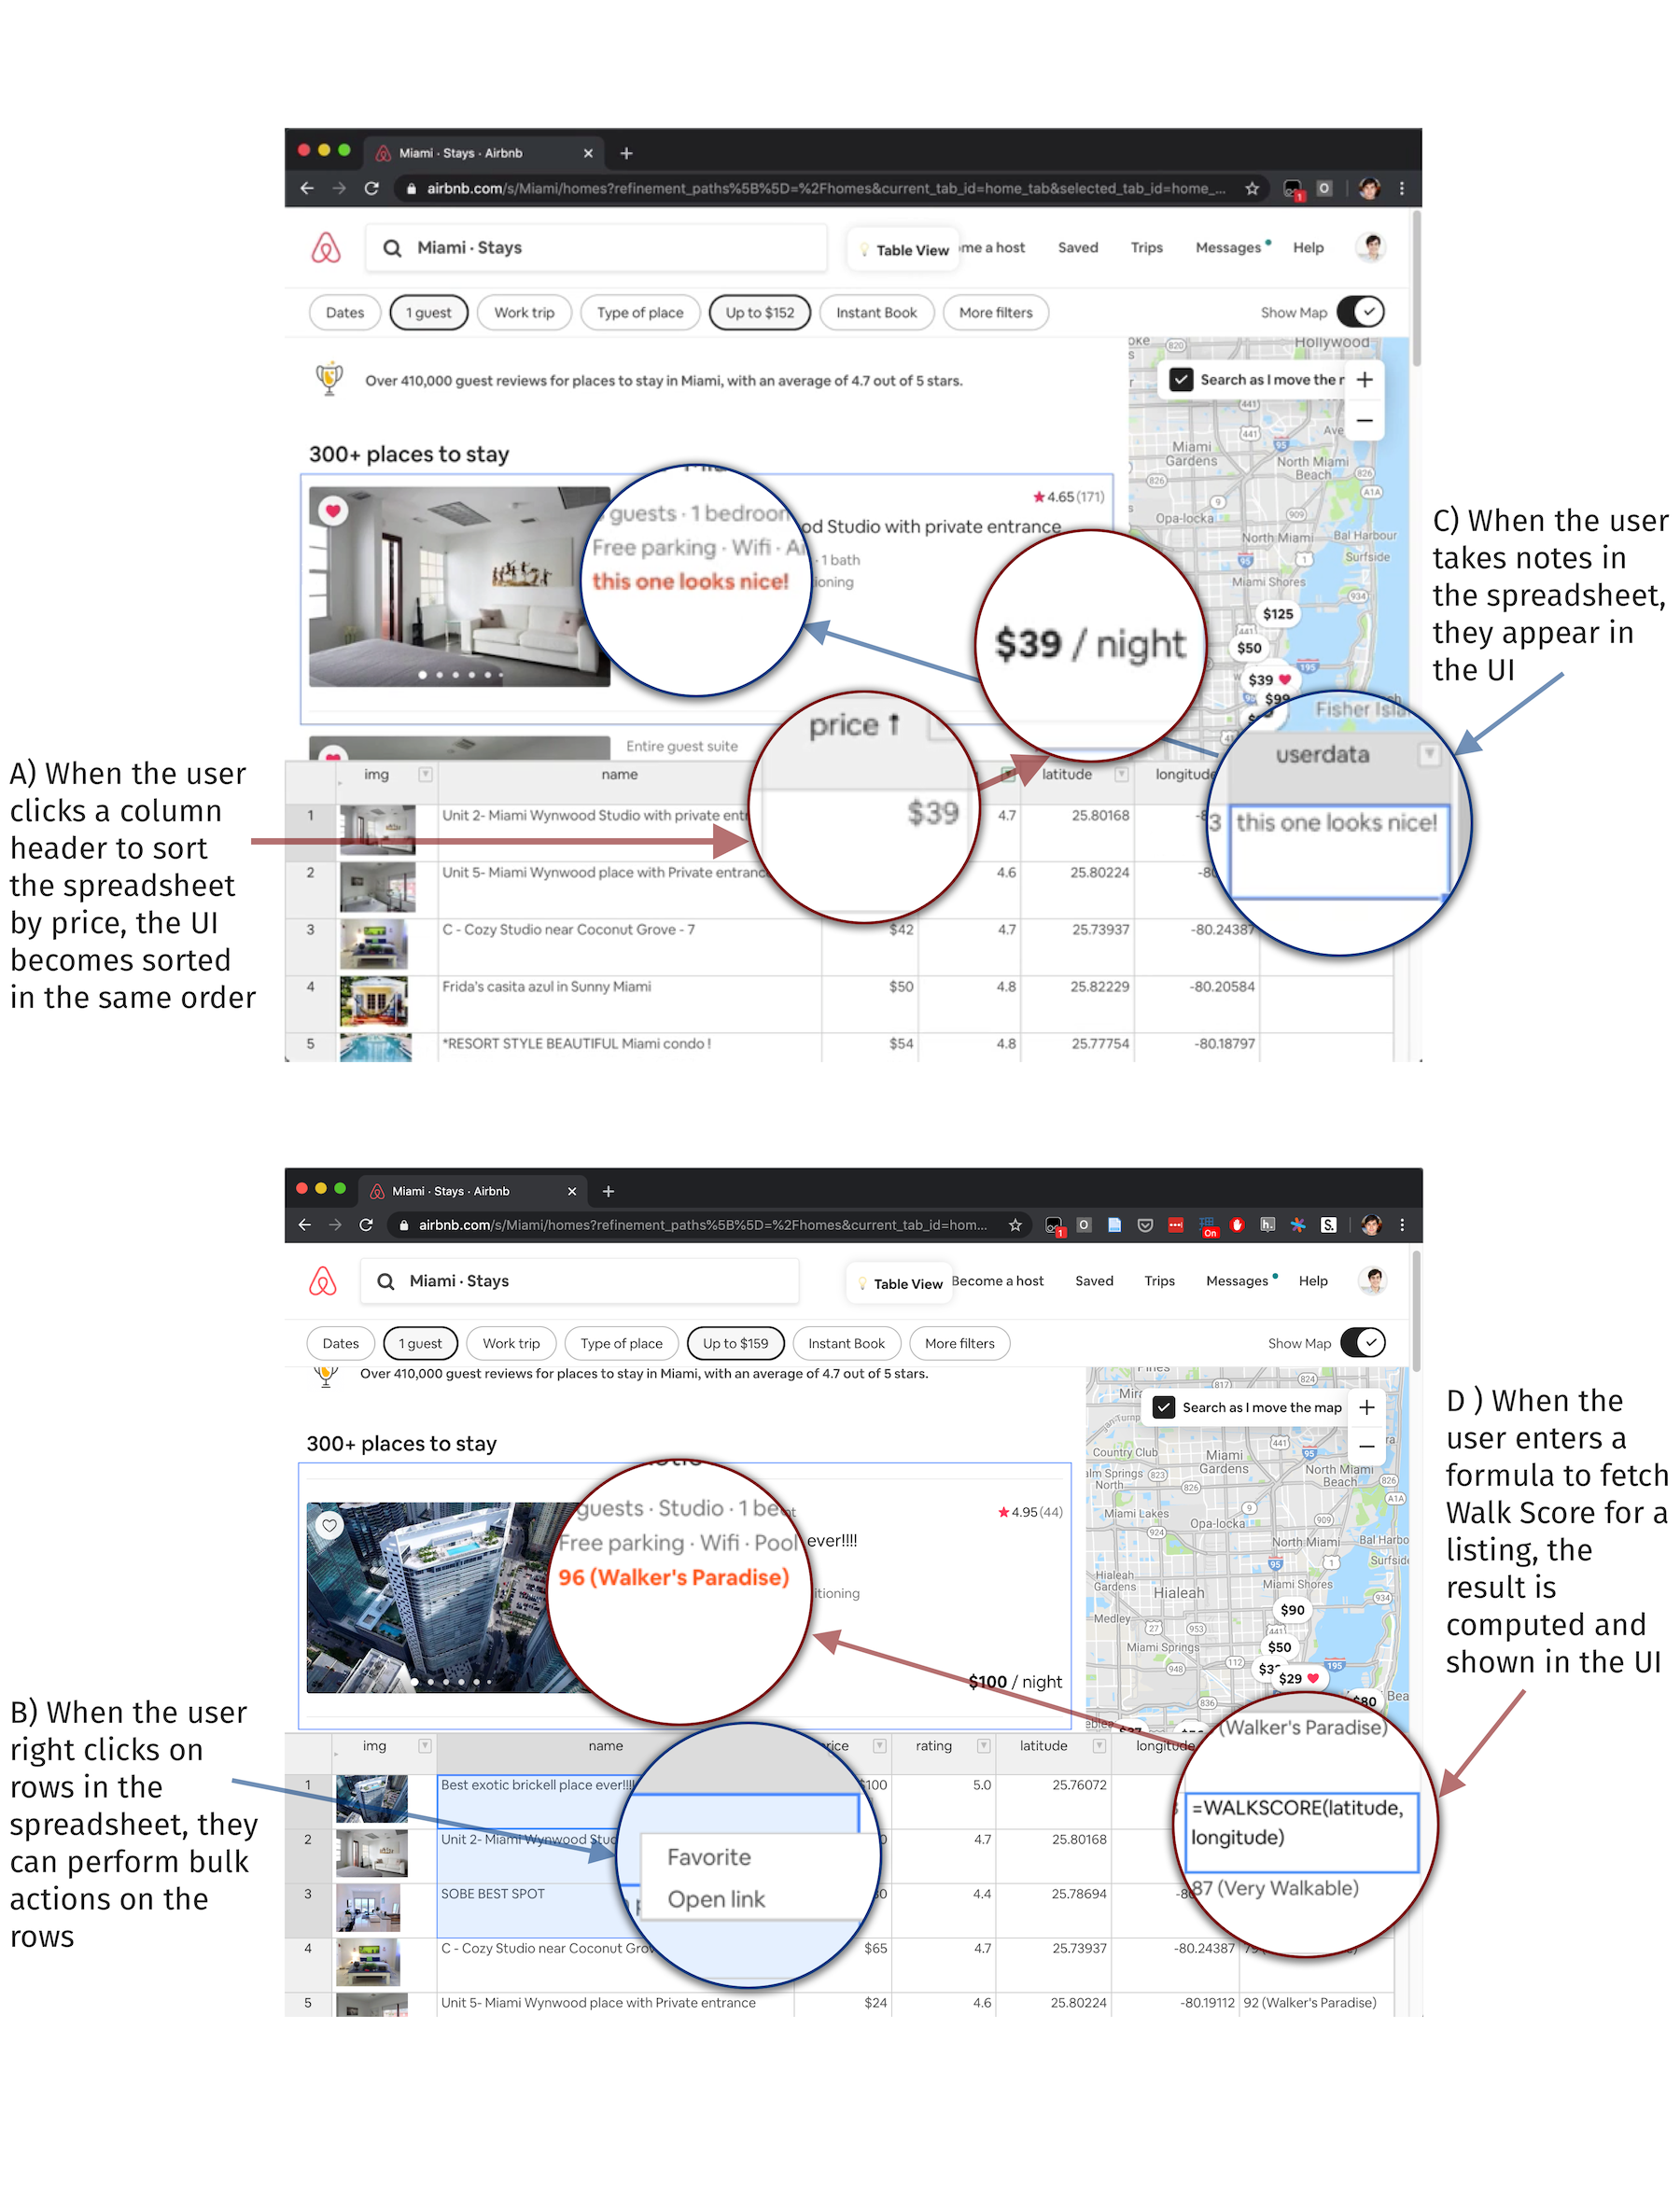
\includegraphics{media/airbnb-demo-300dpi.png}
\caption{Using Wildcard to augment the Airbnb search page for booking
accommodations}\label{fig:airbnb-demo}
}
\end{figure*}

\hypertarget{augmenting-search-results}{%
\subsection{Augmenting search results}\label{augmenting-search-results}}

In 2012, the travel site Airbnb removed the ability to sort
accommodation searches by price. Users could still filter by price
range, but could no longer view the cheapest listings first. Many users
complained that the change seemed hostile to users. ``It's so
frustrating! What is the logic behind not having this function?'' said
one user on the
\href{https://community.withairbnb.com/t5/Hosting/Sorting-listing-by-price/td-p/559404}{Airbnb
support forum}. Alas, the feature remains missing to this day.

Using Wildcard, the user can fix this omission, while leaving the page's
design and the rest of its functionality unchanged.{
Figure~\ref{fig:airbnb-demo} shows an overview of augmenting the Airbnb
site.} First, the user opens up the Wildcard panel, which shows a table
corresponding to the search results in the page. As they click around in
the table, the corresponding row in the page is highlighted to indicate
the mapping between the views.

Then, the user clicks on the price column header to sort the spreadsheet
and the Airbnb UI by price{ (Figure~\ref{fig:airbnb-demo}, Note A)}.
They also filter to listings with a user rating above 4.5 (another
feature missing in the original Airbnb UI).

After manipulating the data, the user closes the table view and
continues using the website. Because the application's UI usually has a
nicer visual design than a spreadsheet, Wildcard does not aim to replace
it---at any time, the user can use either the UI, the spreadsheet, or
both together.

Many websites that show lists of data also offer actions on rows in the
table, like adding an item to a shopping cart. Wildcard has the ability
to make these ``row actions'' available in the data table through the
site adapter. In the Airbnb UI, saving multiple listings to a Favorites
list requires tediously clicking through them one by one. Using Wildcard
row actions, the user can select multiple rows and favorite all of them
with a single click{ (Figure~\ref{fig:airbnb-demo}, Note B)}. Similarly,
the user can open the detailed pages for many listings at once.

Next, the user wants to jot down some notes about each listing. To do
this, they type some notes into an additional column in each row, and
the notes appear inside the listings in the original UI{
(Figure~\ref{fig:airbnb-demo}, Note C)}. The annotations are saved in
the browser and associated with the backend ID of the listing, so they
will appear in future browser sessions that display the same listing.

Wildcard also includes a formula language that enables more
sophisticated customizations. When traveling without a car, it's useful
to evaluate potential places to stay based on how walkable the
surroundings are. Using a formula, the user can integrate Airbnb with
Walkscore, an API that rates the walkability of any location on a 1-100
scale. When the user calls the \texttt{walkscore} formula with the
listing's latitude and longitude as arguments, it returns the walk score
for that location and shows it as the cell value. Because the cell's
contents are injected into the page, the score also appears in the UI{
(Figure~\ref{fig:airbnb-demo}, Note D)}.

\hypertarget{snoozing-todos}{%
\subsection{Snoozing todos}\label{snoozing-todos}}

\begin{figure*}
\hypertarget{fig:airbnb-demo}{%
\centering
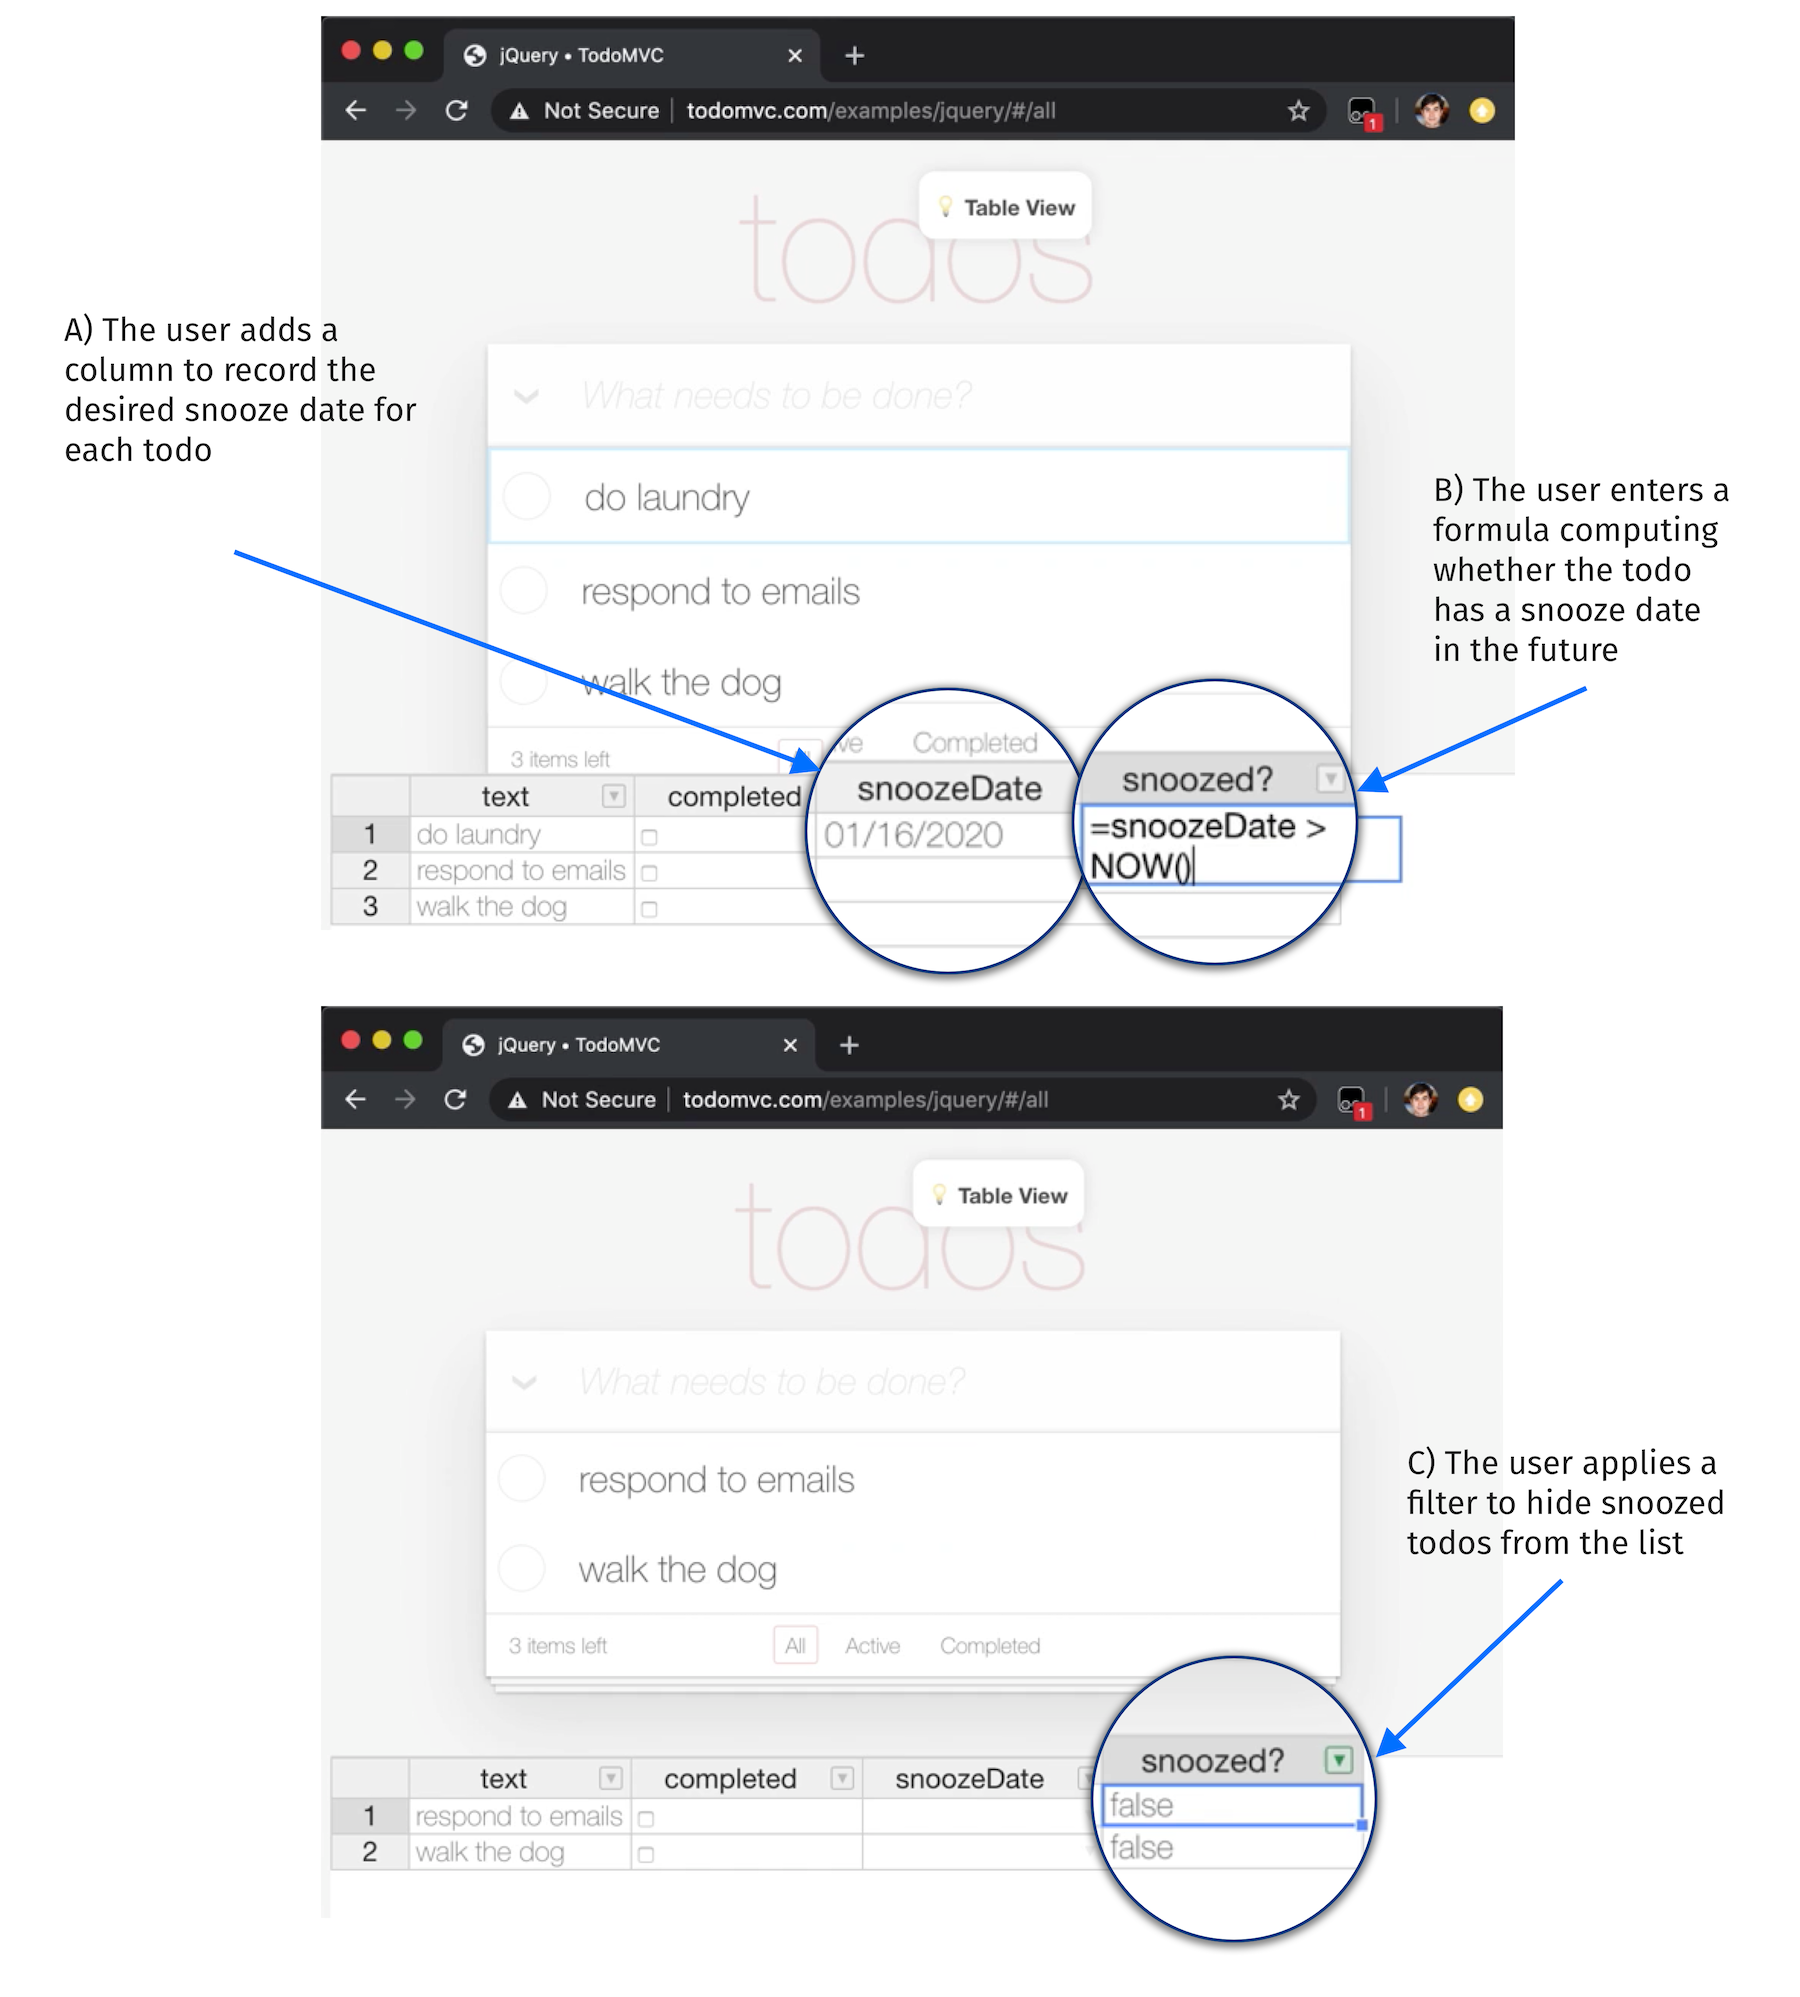
\includegraphics{media/todomvc-demo-300dpi.png}
\caption{Using Wildcard to add a "snooze" feature to the TodoMVC todo list app}\label{fig:todomvc-demo}
}
\end{figure*}

In addition to fetching data from other sources, Wildcard formulas can
also perform computations. In this example, the user would like to
augment the TodoMVC todo list app with a ``snooze'' feature, which will
temporarily hide a todo from the list until a certain date.{
Figure~\ref{fig:todomvc-demo} shows an overview of this customization.}

The user opens the table view, which shows the text and completed status
of each todo. They start the customization by adding a new column to
store the snooze date for each todo{ (Figure~\ref{fig:todomvc-demo},
Note A)}.

The next step is to hide snoozed todos. The user creates a
\texttt{snoozed?} column, which uses a formula to compute whether a todo
is snoozed---i.e., whether it has a snooze date in the future{
(Figure~\ref{fig:todomvc-demo}, Note B)}. Then, they simply filter the
table to hide the snoozed todos{ (Figure~\ref{fig:todomvc-demo}, Note
C)}.

Because the built-in \texttt{NOW()} function always returns the current
datetime, snoozed todos will automatically appear once their snooze date
arrives.

Because this implementation of snoozing was built on the spreadsheet
abstraction, it is completely decoupled from this particular todo list
app. We envision that users could share these types of customizations as
generic browser extensions, which could be applied to any site supported
by Wildcard with no additional effort.

\hypertarget{adding-a-custom-datepicker}{%
\subsection{Adding a custom
datepicker}\label{adding-a-custom-datepicker}}

\begin{figure*}
\hypertarget{fig:airbnb-demo}{%
\centering
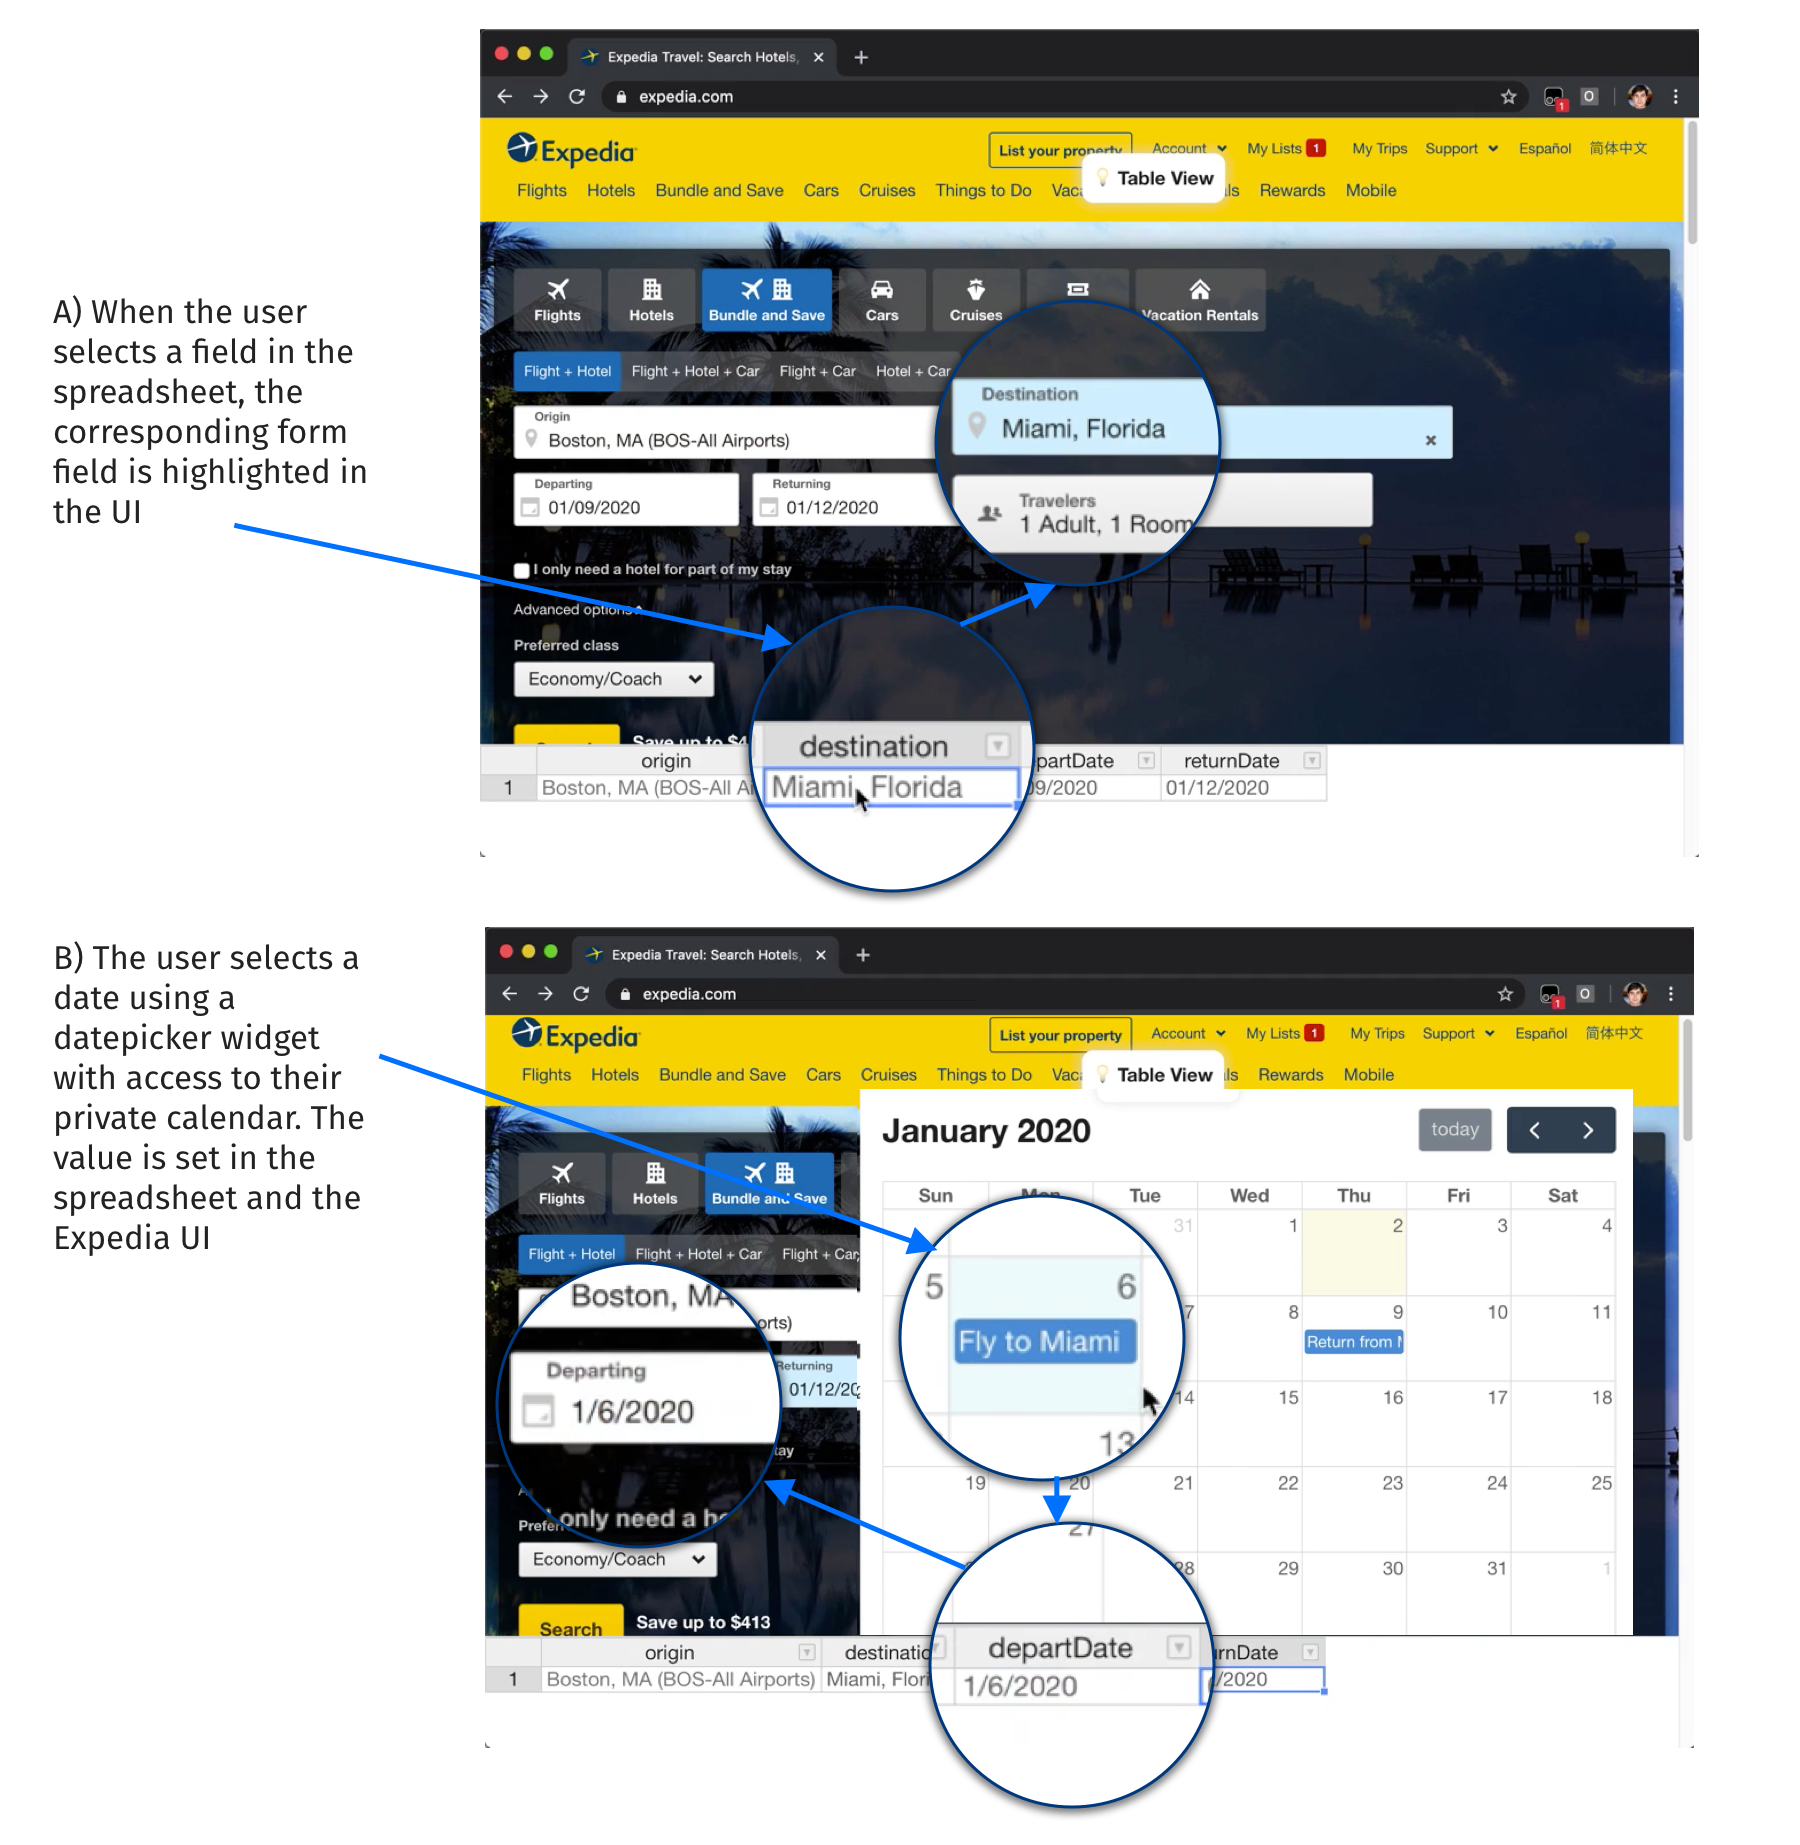
\includegraphics{media/expedia-demo-300dpi.png}
\caption{Using Wildcard to augment the Expedia page for booking a flight}\label{fig:expedia-demo}
}
\end{figure*}

It might seem that Wildcard is only useful on websites that display
lists of tabular data, but the table metaphor is flexible enough to
represent many types of data. For example, a flight search form on
Expedia can be represented as a single row, with a column corresponding
to each input{ (Figure~\ref{fig:expedia-demo}, Note A)}.

In some of the previous examples, the table cells were read-only
(because users can't, for example, change the name or price of an Airbnb
listing). In this case, the cells are writable, which means that changes
in the table are reflected in the form inputs. This becomes especially
useful when combined with GUI widgets that can edit the value of a table
cell.

Filling in dates for a flight search often requires a cumbersome
workflow: open up a separate calendar app, find the dates for the trip,
and then carefully copy them into the form. In Wildcard, the user can
avoid this by using a datepicker widget that shows the user's personal
calendar events{ (Figure~\ref{fig:expedia-demo}, Note B)}. The user can
directly click on the correct date, and it gets inserted into both the
spreadsheet and the original form.n

\hypertarget{sec:architecture}{%
\section{System architecture}\label{sec:architecture}}

\begin{figure}
\hypertarget{fig:table-adapter}{%
\centering
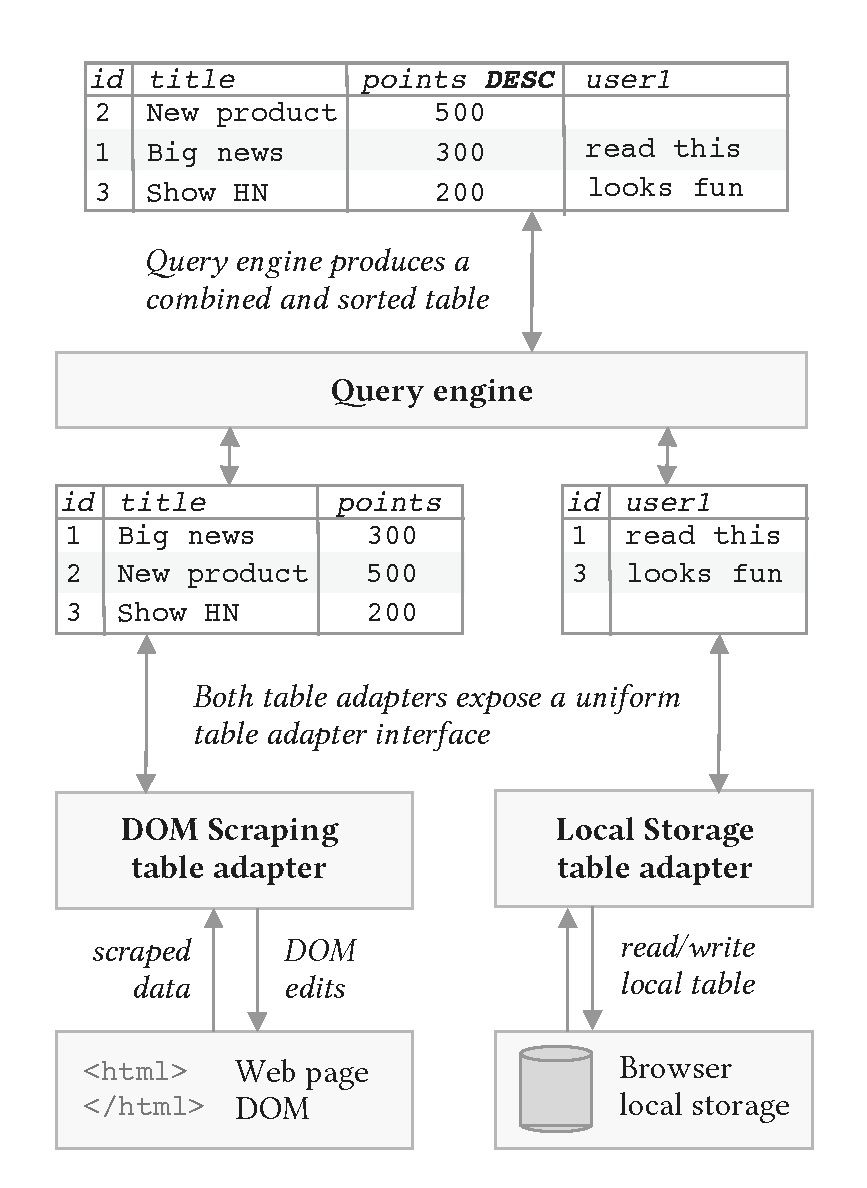
\includegraphics[width=\columnwidth]{media/table-adapter.eps}
\caption{The table adapter architecture}\label{fig:table-adapter}
}
\end{figure}

Figure~\ref{fig:table-adapter} summarizes the overall architecture of
table-driven customization, using a simplified version of the Airbnb
example above. In this example, the name of each listing is scraped from
the web page DOM, the latitude and longitude of each listing is scraped
from AJAX responses, and user annotations are loaded from the brower's
local storage.

First, the three different data sources are each bidirectionally mapped
to a table interface by a \textbf{table adapter}. The table adapter
defines how to map a particular type of data to a table, and what
effects edits should have on the original data source. In some cases,
the mapping logic is straightforward: the local storage adapter stores a
table of data, so the mapping to the table abstraction is trivial. In
other cases, the mapping is more involved: the DOM scraping adapter
implements web scraping logic to produce a table of data from the web
page, and turns edits to the table into DOM manipulations like
reordering rows of data on the page.

The three separate tables are then combined into a single table for the
end user to view and edit. The \textbf{query engine} is responsible for
creating this combined view, and routing the user's edits back to the
individual table adapters. In this example, the query engine has joined
the three tables together by a shared ID column, and sorted the result
by the name column.

We now examine each component of the system in more detail.

\hypertarget{table-adapters}{%
\subsection{Table adapters}\label{table-adapters}}

A key idea in table-driven customization is that a wide variety of data
sources can be mapped to the generic abstraction of an editable table.
In a relational database, the table matches the underlying storage
format, but in table-driven customization, the table is merely an
\emph{interface layer}. The data shown in the table is a projection of
some underlying state, and edits to the table can have complex effects
on the underlying state.

Externally, a table adapter must satisfy an abstract interface. The
first two parts of the interface resemble the interface exposed by a
table in a relational database:

\textbf{Returning a table}: A table adapter exposes a table of data: an
ordered list of records. Each record carries a unique identifier and
associates named attributes with values. Tables have a typed schema, so
the same attributes are shared across all records. A table adapter can
update the contents of a table at any time, in response to changes in
the underlying state (e.g., a DOM scraping adapter can update the table
when the page body changes). When data changes, the query view is
reactively updated in response.

\textbf{Making edits}: The query engine can issue a request to a table
adapter to make an edit to a record. The meaning of making an edit can
vary depending on the adapter: in the local storage adapter, an
annotation may be persisted into local storage; in the DOM scraping
adapter, an edit may represent filling in a form field. An adapter can
also mark values as read-only if it wouldn't be meaningful to edit them;
for example, the DOM scraping adapter typically marks page content as
read-only, except for editable form fields.

The query engine also sends additional information about the combined
query view to each table adapter. These functions are currently used to
provide the DOM scraping adapter with sufficient information to
manipulate the original application UI as the user manipulates the table
view.

\textbf{Sorting/filtering}: When the user sorts or filters the query
view, an ordered list of visible IDs is sent to each table adapter. The
DOM scraping adapter uses this information to modify the list of visible
rows in the web page.

\textbf{Information from other tables}: The query engine sends each
table adapter the entire combined table of data being rendered to the
user. The DOM scraping adapter uses this to add annotations to the page
by looking for additional data columns joined to scraped rows, and
rendering them in the page.

\textbf{Currently selected record}: The query engine notifies each table
adapter about which record is currently selected by the user in the
table UI. The DOM scraping adapter uses this information to highlight
the row in the page that corresponds to the selected record in the
table.

\hypertarget{types-of-table-adapters}{%
\subsubsection{Types of table adapters}\label{types-of-table-adapters}}

Here we describe in more detail the table adapters that we have
implemented in Wildcard to power the customizations shown in
Section~\ref{sec:examples}.

\textbf{DOM scraping adapters} are the essential component that enables
Wildcard to interface with an existing website UI. In addition to the
standard web scraping problem of extracting a table of data from the
DOM, a scraping adapter must also manipulate the DOM to reorder rows,
edit form entries, and inject annotations as the table is edited.

Because each website has unique content, we rely on programmers to
create a DOM scraping adapter for each individual website to make it
available for customization in Wildcard. To make this approach viable,
we have built a library of functions that make it easy to implement a
scraping adapter, requiring the programmer only to implement the minimal
site-specific parts. The programmer writes a single Javascript function
which can use standard scraping techniques like CSS selectors and DOM
APIs to extract relevant elements from the page. The library functions
then wrap this function to implement the rest of the needed
functionality; for example, when the table is sorted, we find the DOM
elements corresponding to the rows in the table, remove them from the
page, and then reinsert them in the new order.

An \textbf{AJAX scraping adapter} intercepts AJAX requests made by a web
page, and extracts information from those requests. When available, this
tends to be a helpful technique because the data is already in a
structured form, and often includes information not shown in the UI. As
with DOM scraping adapters, we have made it easy for programmers to
create site-specific AJAX scraping adapters. A programmer writes a
function that specifies how to extract data from an AJAX request, and
the framework handles the details of intercepting requests and calling
the programmer-defined function.\footnote{So far we have only
  implemented AJAX scraping in the Firefox version of Wildcard, since
  Firefox has convenient APIs for intercepting requests. It appears
  possible to implement in Chrome as well, but we have not finished our
  implementation.}

The \textbf{local storage adapter} simply stores a table of data in the
browser. As shown in the example use cases, this can be useful for
persisting annotations in a private way, without uploading them to a web
service.

\hypertarget{future-adapters}{%
\subsubsection{Future Adapters}\label{future-adapters}}

We have designed the table adapter API to be general enough to support
other types of useful adapters in the future. Here are two such
possibilities:

\textbf{Integrated website adapters}: A key benefit of the table adapter
abstraction is that Wildcard is not coupled to web scraping as the only
means for integrating with existing sites, but can also accommodate
first party developers adding support directly into their own websites.
An ``integrated website adapter'' installed by the developer could
directly accesses the internal state of the application, providing the
same functionality as a DOM scraping adapter but in a more robust way.

With the advent of rich frontend web frameworks, structured application
state is now often available in the web client. We suspect it is
possible to create plugins for frontend frameworks that expose this
state to Wildcard with only minimal effort from the application
developers. To test this hypothesis, we have created an early prototype
of a Wildcard adapter for the Redux state management library, and used
it with the TodoMVC todo list application. To install the adapter, the
programmer only needs to make a few small changes to their app:

\emph{Exposing a table}: In Redux, app developers already represent the
state of a user interface as a single object. To expose a table of data,
the developer simply writes a function that maps the state object to a
table. \emph{Editing data values}: The developer defines how edits to
records in the table should map to edits in the state object.
\emph{Sorting/filtering the UI}: The developer inserts an additional
data processing step before the state object is rendered in the UI, so
that Wildcard can apply sorting and filtering. \emph{Annotations}: The
developer adds additional React components managed by Wildcard into
their UI tree, which render additional data as annotations.

In certain types of software, customizability is often touted as a key
selling point. An integrated website adapter would provide a way for
developers to integrate with an existing ecosystem of formulas and
customization tools, without needing to build all that functionality
from scratch.

\textbf{Shared storage adapter}: It would be useful to share user
annotations among users and across devices---for example,
collaboratively taking notes with friends on options for places to stay
on Airbnb. The existing Local Storage Adapter could be extended to share
live synchronized data with other users. This could be achieved through
a centralized web server, or through P2P connections that might provide
stronger privacy guarantees.

\hypertarget{query-engine}{%
\subsection{Query engine}\label{query-engine}}

The query engine is responsible for coordinating across multiple table
adapters. It joins data across multiple tables and creates a single
result table which is shown to the user through the editor. It also
handles all user interactions and routes appropriate messages to each
table adapter.

Queries are processed in three steps. First, the query invokes a primary
DOM scraping table adapter that associates records in the result with
elements in the application's user interface. At minimum, the primary
table adapter needs to return record IDs and have the ability to
manipulate the application's UI. It can also optionally return data
about each record. Next, additional tables (AJAX data, local storage
data) are left-joined by ID. Finally, the result table can be sorted and
filtered by any column.

This query model can be viewed as a tiny (and rather constrained) subset
of the SQL query model. Despite its simplicity, this simple model has
proven sufficient for meeting the needs of customization in practice,
and minimizes the complexity of supporting more general and arbitrary
queries. But because it fits into the general paradigm of relational
queries, it could theoretically be extended to support a wider range of
queries.

The query engine is also responsible for executing formulas. We have
built a small formula language resembling the ones used in visual query
tools like SIEUFERD. As in those tools, and unlike in spreadsheets,
formulas automatically apply across an entire column of data, and
reference other column names instead of values on specific rows. For
example, the user would write \texttt{=price\ *\ 2} to create a column
with a value derived from a price attribute. This is more convenient
than needing to copy-paste a formula across an entire column as in
spreadsheets, and none of our customization use cases have uncovered a
need for writing different formulas on different rows of the table.

\hypertarget{table-editor}{%
\subsection{Table editor}\label{table-editor}}

In Wildcard we provide a basic table editor as the user interface on top
of the query engine. It is built with the Handsontable Javascript
library, which provides UI elements for viewing and editing a table, as
well as basic query operations like sorting and filtering.

\emph{todo: other table instruments}

\begin{table*}[]
\begin{tabular}{llrl}
\hline
\textbf{Website} & \textbf{Description} & \textbf{LOC} & \textbf{Example customizations}                                                              \\ \hline
Airbnb           & Travel               & 73                                       & Add Walkability Scores to listings. Sort listings by price.                           \\
Amazon           & Online shopping      & 99                                       & Sort used book sellers by total price, including delivery fees                                \\
Blogger          & Blogging             & 36                                       & Use alternate text editor to edit blog posts                                                 \\
Expedia          & Travel               & 41                                       & Use alternate datepicker to enter travel dates                                               \\
Flux             & Data portal          & 67                                       & Use Wildcard as a faster table editor for editing lab results                                \\
Github           & Code repository      & 62                                       & Sort a user's code repositories by stars to find popular work                                \\
Hacker News      & News                 & 69                                       & Add read times to links. Filter out links that have been read. \\
Instacart        & Grocery delivery     & 48                                       & Sort groceries by price and category. Take notes on items.                                   \\
Uber Eats        & Food delivery        & 117                                      & Sort/filter restaurants by estimated delivery ETA and price.                                 \\
Weather.com  & Weather              & 51                                       & Sort/filter hourly weather to find nice times of day.                                        \\
Youtube          & Videos               & 80                                       & Sort/filter videos by length, to find short videos to watch.                                 \\ \hline
\end{tabular}
\caption{A list of table-driven customizations that we have implemented using Wildcard.}
\label{tab:websites}
\end{table*}

\hypertarget{sec:evaluation}{%
\section{Evaluation}\label{sec:evaluation}}

To evaluate table-driven customization in practice, we built the
Wildcard browser extension, which implements table-driven customization
in the context of existing websites. It is built in Typescript, and
works across three major browsers: Chrome, Firefox, and Edge.

We have used Wildcard to customize 11 websites, including transactional
sites like Amazon and Uber Eats, and media consumption sites like Hacker
News and Youtube. Table 1 summarizes all these customizations, including
the number of lines of code in the adapter configuration for each site.

So far, most usage of Wildcard has come from members of the project
team. Here we offer our reflections on using the system, focused on two
key questions:

\begin{itemize}
\tightlist
\item
  How broad is the range of possible customizations in this paradigm?
\item
  How feasible is it to build DOM scraping adapters for real websites,
  in practice?
\end{itemize}

\hypertarget{range-of-customizations}{%
\subsection{Range of customizations}\label{range-of-customizations}}

We have found that table-driven customization can serve a broad range of
useful purposes. Here we expand on some examples that illuminate various
aspects of using the system in practice.

\hypertarget{sortingfiltering}{%
\subsubsection{Sorting/filtering}\label{sortingfiltering}}

It might seem that most websites already have adequate sorting and
filtering functionality, but we have found it surprisingly helpful to
add new sorting/filtering functionality to websites using Wildcard.

Sometimes, websites have opaque algorithms which they use to rank
results, which presumably maximize profit but don't offer much control
to the user. For example, Airbnb doesn't allow users to sort listings by
price, and Youtube doesn't allow users to sort the homepage by watch
time. Wildcard enables users to take back some control over this
process.

In other cases we have found that a lack of sorting options seems less
intentional, and simply a missing feature. For example, the Instacart
grocery delivery service doesn't allow users to sort their grocery cart
by price or category. Our guess is that they simply haven't gotten
around to implementing the feature yet.

In the current implementation of Wildcard, users can only sort and
filter entries which are shown on the current page, which means that
users are not entirely liberated from the suggestions of the opaque
algorithm. We could work around this restriction in the future by
fetching content across multiple pages, but we've also found that
sorting/filtering a single page of a paginated list is often an
acceptable outcome, and even a preferable one. For example, it's more
useful to sort 30 recommended Youtube videos than to try to sort all
videos on Youtube; similarly it's convenient to view the Hacker News
front page sorted by read time, rather than all Hacker News articles.

\hypertarget{annotating}{%
\subsubsection{Annotating}\label{annotating}}

Many other web annotation systems focus on annotating text or arbitrary
webpage content, but Wildcard only allows for annotating structured
objects extracted by an adapter, which results in quite a different set
of use cases.

Annotating with Wildcard has proven most useful when taking notes on a
list of possible options: e.g., evaluating possible Airbnb locations to
rent. We have also used it with Instacart's online grocery cart, for
jotting down notes like ``should we get more milk?''

\hypertarget{formulas}{%
\subsubsection{Formulas}\label{formulas}}

Formulas are the most powerful part of the Wildcard system. So far, we
have only built a small number of functions into the language, but by
adding more functions, the fundamental computing model could support a
very broad range of useful computations, as shown by the success of
spreadsheets.

We have found that formulas are useful for fetching data from Web APIs.
We've used them to augment Airbnb listings with walkability scores, and
augment Hacker News articles with estimated read times. One challenge of
the current language design is that supporting each web API requires
adding a new function to the language using code, because web APIs
typically return complex JSON data structures which don't make sense to
display in a single table cell. Adding functions for handling JSON data
to the formula language might help resolve this.

We have also found instances where simple data manipulation is useful:
adding together different subtotals into a total price, or manipulating
the results of a formula expression with arithmetic or concatenating
string labels, as shown in the example in Section~\ref{sec:examples}.
(\emph{todo: this makes sense iff we switch the examples sectino to HN})

\hypertarget{cell-editors}{%
\subsubsection{Cell editors}\label{cell-editors}}

(\emph{note: written with the assumption that Expedia gets cut from the
Examples section})

``Cell editors'' are UI widgets that expose a custom editing UI for a
single cell of the table view. A programmer building a cell editor only
needs to integrate it with the table viewer; actually propagating values
into the website UI is handled by the site-specific DOM adapter. As a
result, creating a new cell editor can be as easy as just creating glue
code between the table editor and an existing UI widget library.

One benefit of cell editors is that a user can use their personal
information in a web UI without uploading it to the website. To explore
this idea, we created a cell editor based on the FullCalendar Javascript
plugin, which can load data from a Google Calendar. This makes it
convenient to enter dates into a website based on the user's personal
calendar information.

Another benefit of cell editors is that a user can choose their
preferred widget for editing some type of information. We built a cell
editor based on the CKEditor rich text editor. As an example of using
this editor, we integrated it with the Blogger website and used it to
edit blog posts, in place of the Blogger website's built-in editor.

\hypertarget{limitations}{%
\subsubsection{Limitations}\label{limitations}}

There are many useful customizations which are not possible in the
table-driven customization paradigm. Wildcard can only make
customizations that use the available data exposed in the table. UI
modifications are limited in scope; for example, deleting arbitrary
buttons isn't possible. At one point, we wanted to build an automation
to repeatedly load a grocery delivery website to check for open delivery
slots, but it wasn't clear how to achieve this. Some of these
limitations are specific to the current implementation of the Wildcard
extension, but some are more general to the entire idea of table-driven
customization.

We consider this an acceptable outcome---our goal is simply to make many
useful customizations available to end users with a low threshold, not
to span all possible customizations. Section~\ref{sec:dm} discusses this
point further.

One benefit of Wildcard is \emph{predictability}: once we built a site
adapter for a website, it was generally obvious to us what types of
customizations were and weren't possible, and the UI guided us towards
building customizations that matched the system's model. For example,
it's clear that it's not possible to customize a website using data not
available in the table.

\hypertarget{viability-of-dom-scraping}{%
\subsection{Viability of DOM scraping}\label{viability-of-dom-scraping}}

Our second evaluation area is less about the conceptual approach of
table-driven customization, and more about our specific implementation
of customizing existing web applications. In order for third-party
customization through Wildcard to succeed, it is important that creating
usable adapters for existing websites takes minimal effort.

Most of our DOM scraping adapters were created by members of our team.
However, an external developer unaffiliated with the project contributed
one adapter, designed to sort the Github page listing a user's
repositories. They described the experience as ``very straightforward.''

The adapters for our test sites ranged from 36 to 117 lines of code,
averaging 68 lines; Table 1 shows the full lines of code for each
adapter.

Some of the challenges of writing a DOM scraping adapter are the same
ones as with writing normal web scraping code, but the more interactive
nature of Wildcard introduces additional challenges. rve changes, but it
may prove challenging to observe changes on some sites only through the
DOM. One challenge is triggering updates to the spreadsheet data in
response to UI changes that happen after initial page load. Site
adapters are responsible for recognizing these changes by observing the
DOM. So far, we have been able to use event listeners and the
MutationObserver API to successfully obse

Another challenge is persisting updates to the DOM---some websites use
virtual DOM frameworks that can occasionally overwrite changes made by
Wildcard.

So far, we've managed to work around these issues for all the websites
we've tried, but we don't claim that any website can be customized
through DOM scraping. As web frontend code gets increasingly complex
(and starts to move beyond the DOM to other technologies like Shadow DOM
or even WebGL for rendering), it may become increasingly difficult to
customize websites from the outside without first-party support.

\hypertarget{sec:themes}{%
\section{Key themes}\label{sec:themes}}

\hypertarget{sec:dm}{%
\subsection{Customization by direct manipulation}\label{sec:dm}}

Hutchins, Hollan and Norman \citep{hutchins1985} describe a direct
manipulation interface as one that uses a model-world metaphor, rather
than a conversation metaphor. Rather than conversing with the system
about an assumed world, ``the world is explicitly represented'' and the
user can ``{[}act{]} upon the objects of the task domain themselves.''

Most GUIs today employ direct manipulation, but software customization
tools typically use an imperative programming model, which implements
the conversational metaphor rather than direct manipulation. For
example, in Applescript \citep{cook2007}, the scripting language for
customizing Mac OS applications, here is how a user retrieves a list of
of calendar names from the Calendar application:

\begin{verbatim}
tell application "Calendar"
  name of calendars
end tell
\end{verbatim}

Some customization environments (Automator for Mac, Shortcuts for iOS,
Zapier for web APIs) forego text syntax and enable the user to connect
programs and construct automations by dragging and dropping commands.
These environments still do not constitute direct manipulation, though:
the objects being manipulated are in the domain of programming, not the
domain of the task at hand.

Imperative programming is a reasonable choice as the model for building
customizations. Turing-complete programming provides a high ceiling for
possible customizations, and a sequence of commands is a natural fit for
automations which simulate a series of steps taken by the user.

However, there is a serious drawback to this approach. MacLean et al
\citep{maclean1990} describe an ideal for user-tailorable systems: a
``gentle slope'' from using to customizing, where small incremental
increases in skill lead to corresponding increments of customization
power. Requiring users to learn programming for customization creates an
abrupt ``cliff,'' where a significant learning investment is required
even to implement simple customizations. Another goal of MacLean et al
is that ``it should be as easy to change the environment as it is to use
it,'' at least for some subset of changes. In scripting languages, even
user-friendly ones like Applescript or Chickenfoot, the experience of
customization does not remotely resemble the experience of use, so these
systems can't meet this goal.

With table-driven customization we aim to provide a gentler slope, by
using direct manipulation for software customization. The data shown in
the table view is the domain data from the original application. The
user makes changes to the data by selecting areas of interest in the
table, e.g.~sorting/filtering by clicking the relevant column header, or
adding annotation by clicking on the relevant row. These interactions
are common in GUI applications, and Wildcard therefore meets MacLean et
al's goal: some one-click customizations are as easy as using the
original application.

One aspect of directness which we have chosen not to maintain in
Wildcard is enabling customization in the context of the original user
interface, as explored by some other tools like Scotty
\citep{eagan2011}. We have found that augmenting the original UI with an
additional structured representation has numerous benefits. It provides
a consistent experience across all applications, and clearly shows the
user what structured data is available to work with.

Ainsworth et al provide a helpful taxonomy of the value of multiple
representations \citep{ainsworth1999}. In their terms, Wildcard plays a
\emph{complementary role} by supporting a different set of tasks from
the original application, while displaying \emph{shared information}. We
also suspect that Wildcard helps \emph{constructs deeper understanding}
by \emph{subtraction}. By stripping away details and only showing the
essential data in an interface, Wildcard helps users think of new ways
of using that data, outside the specific constraints of the original
application.

It is important to note that there are many specific customizations that
can be achieved in systems like Chickenfoot \citep{bolin2005} that
cannot be reproduced in Wildcard. We consider this an acceptable
tradeoff in exchange for achieving a gentler slope of customization, and
we show in Section~\ref{sec:examples} and Section~\ref{sec:evaluation}
that our model can still implement many useful customizations in
practice. Also, there is sometimes a way to reframe an imperative script
in terms of our direct manipulation model; for example, a script that
iterates through rows in a page adding some additional information could
be reproduced using a formula in Wildcard.

\hypertarget{wrapping-applications-for-customization}{%
\subsection{Wrapping applications for
customization}\label{wrapping-applications-for-customization}}

Software customization tools typically fall into one of two categories:
third-party, or semantic.

\emph{Ad hoc customization tools} enable customization without using
official extension APIs, enabling a broader range of customizations on
top of more applications. For example, web browser extensions have
demonstrated the utility of customizing websites through manipulating
the DOM, without needing explicit extension APIs to be built in.
However, ad hoc customization comes with a corresponding cost: these
tools can typically only operate at a low level of abstraction,
e.g.~manipulating user interface elements. This makes it harder for end
users to write scripts, and makes the resulting scripts more brittle.

\emph{Anticipated customization tools}, in contrast, use explicit
extension APIs provided by the application developer. Examples of this
include accessing a backend web API, or writing a customization in
Applescript that uses an application-specific API. The main benefit is
that this allows the extension author to work with meaningful concepts
in the application domain---``create a new calendar event'' rather than
``click the button that says new event.''---which makes customizations
easier to build and more robust. However, this style limits the range of
extensions that can be built to those that the official plugin API
supports.

With Wildcard, we use a hybrid approach that aims to provide the best of
both worlds. Programmers implement an API wrapper that is internally
implemented as an ad hoc customization, but externally provides a
high-level interface to the application, abstracting away the details of
the user interface. These wrappers are added to a shared repository,
available to all users of the system. When an end user is using a site
that already has an adapter, they get a semantic customization
experience that avoids low-level details.

One way to view this approach is as introducing a new abstraction
barrier into third-party extension. Typically, a third party
customization script combines two responsibilities: 1) mapping the
low-level details of a user interface to semantic constructs (e.g.,
using CSS selectors to find certain page elements), and 2) handling the
actual logic of the specific customization. Even though the mapping
logic is often more generic than the specific customization, the
intertwining of these two responsibilities in a single script makes it
very difficult to share the mapping logic across scripts.

With Wildcard we propose a decoupling of these two layers: a repository
of shared wrappers maintained by programmers, and a separate repository
of specific customizations built on top of these wrappers. This general
architecture has been successfully demonstrated by projects like
Gmail.js, an open source project that creates a convenient API for
browser extensions to interface with the Gmail web email client.

(\emph{todo: mention automated wrapper induction here or somewhere
else?})

\hypertarget{sec:related-work}{%
\section{Related Work}\label{sec:related-work}}

This paper extends work reported in a workshop paper by Litt and Jackson
\citep{litt2020} which presented an early prototype version of Wildcard.
We have substantially extended their work in this paper by creating the
table adapter abstraction and reimplementing the system around that
abstraction, evaluating the system more fully on many more websites, and
by characterizing the design of the system in more detail.

Table-driven customization relates to two broad areas of related work.
Our problem statement is related to software customization tools, and
our solution approach is related to spreadsheets and other direct
manipulation interfaces.

\hypertarget{customization-tools}{%
\subsection{Customization tools}\label{customization-tools}}

Table-driven customization is most closely related to other tools that
aim to empower end users to customize software without doing any
programming.

This lineage goes back at least to the Buttons system by MacLean et al
\citep{maclean1990}, where Xerox Lisp users could share buttons that
performed various ``tailoring'' actions on the system. The authors
proposed the ``gentle slope'' idea which has greatly influenced our
approach to table-driven customization (as discussed in
Section~\ref{sec:dm}). The authors also point out the importance of a
``tailoring culture'' where people with different skillsets collaborate
to produce useful customizations; in their system, Lisp programmers
create buttons that others can use, modify, and rearrange. This division
of labor corresponds to our idea of semantic wrappers, where end user
customization is supported by programmer-created building blocks.

Some recent web customization tools aim to enable end users to modify
web interfaces without programming.

Sifter \citep{huynh2006} enables end users to sort and filter lists of
data based on web scraping, much like Wildcard's sorting features. The
main difference between the systems is that table-driven customization
has many other use cases besides sorting and filtering. Also, Sifter
involves end users in a semi-automated data extraction process, rather
than having programmers create wrappers. This provides coverage of more
websites, but at the expense of complicating the end user experience. We
might explore such techniques in Wildcard in the future, but we think
that it's valuable for end users to have a customization experience free
of web scraping details on supported websites. Finally Sifter implements
scraping across multiple pages, a valuable feature for sorting and
filtering which isn't present in Wildcard.

Thresher \citep{hogue2005} enables end users to create wrappers which
map website content to Semantic Web schemas, making customizations
available using the schema information. We share the general idea of
wrappers with Thresher, but we have chosen to map to a single generic
data type, rather than more specific schemas, which increases the range
of websites and data supported by the system.

There are many software customization tools that offer simplified
versions of programming for end users. Chickenfoot \citep{bolin2005} and
Coscripter \citep{leshed2008} offer friendly syntax for writing web
automation scripts; Applescript \citep{cook2007} attempts a similar goal
for desktop customization. There are visual programming environments for
customization which don't involve writing any text: as a few examples,
\href{https://support.apple.com/guide/automator/welcome/mac}{Automator}
for Mac and
\href{https://apps.apple.com/us/app/shortcuts/id915249334}{Shortcuts}
for iOS are modern options for customizing Apple products, and
\href{https://zapier.com/}{Zapier} enables users to connect different
web applications together visually. As mentioned previously, these tools
all require writing imperative programs in some form; we take a
fundamentally different approach in table-driven customization.

\hypertarget{direct-manipulation-programming-interfaces.}{%
\subsection{Direct manipulation programming
interfaces.}\label{direct-manipulation-programming-interfaces.}}

Another relevant area of literature is direct manipulation interfaces
for interacting with structured data. We take much inspiration from
these tools in our work, but apply them in a different domain:
customizing existing software applications, rather than interacting with
databases or constructing software from scratch.

The most closely related work is in systems that offer spreadsheet-like
querying of relational data, as proposed by Liu and Jagadish
\citep{liu2009}. SIEUFERD by Bakke and Karger \citep{bakke2016} is an
example; their paper presents a survey of various other similar tools.
Our work is particularly influenced by the authors' observation that
direct manipulation requires that the user manipulate the \emph{results}
of a database query rather than the query itself, and that the user must
see intermediate results at every step of constructing a computation.
SIEUFERD's interface supports a far wider range of possible queries than
Wildcard, but the basic ideas of the user interface are similar.

\href{https://airtable.com/}{Airtable} is another example of a modern
commercial product that offers spreadsheet-like interaction with a
relational database.

Our work is also inspired by the many projects which have explored using
spreadsheets as a foundation for building software applications,
including Object Spreadsheets \citep{mccutchen2016}, Quilt
\citep{benson2014}, Gneiss \citep{chang2014}, Marmite \citep{wong2007},
\href{https://www.glideapps.com/}{Glide}. These projects share the idea
that a spreadsheet is a convenient interface for editing the data
underlying a GUI application. We share that idea, but apply it to
software customization, rather than building software from scratch.

Another system in this space is ScrAPIr, by Alrashed et
al.~\citep{alrashed2020}, which enables end users to access backend web
APIs without programming. ScrAPIr shares a high level goal of end user
empowerment, and also shares the idea of wrappers, by creating a shared
library of wrappers around existing web APIs. However, unlike Wildcard,
ScrAPIr targets explicit APIs exposed by developers, and also doesn't
aim to extend the frontend interfaces of web applications.

\hypertarget{conclusion}{%
\section{Conclusion}\label{conclusion}}

\emph{todo}

%%
%% The next two lines define the bibliography style to be used, and
%% the bibliography file.
\bibliographystyle{ACM-Reference-Format}
\bibliography{wildcard-onward-bibtex.bib}

\end{document}
\endinput
%%
%% End of file `sample-sigconf.tex'.
